\chapter{پیاده‌سازی سخت‌افزاری}
\noindent
\textbf{
	\textit{
	سنتز سیستم روی FPGA 
	، بررسی ایرادات سنتز و ارائه راهکار، گزارش پیاده‌سازی  
	}
}
\pagebreak

\section{مقدمه‌ای بر پیاده‌سازی سخت‌افزاری}
کد verilog داده‌شده در پزوژه با استفاده از ابزار 
Quartus 
برای سنتز بر روی FPGA شبیه‌سازی شد، در ادامه مختصرا به شرح ایرادات سنتز و سپس به گزارش آمارهای حاصل از سنتز می‌پردازیم. 

\begin{figure}[H]
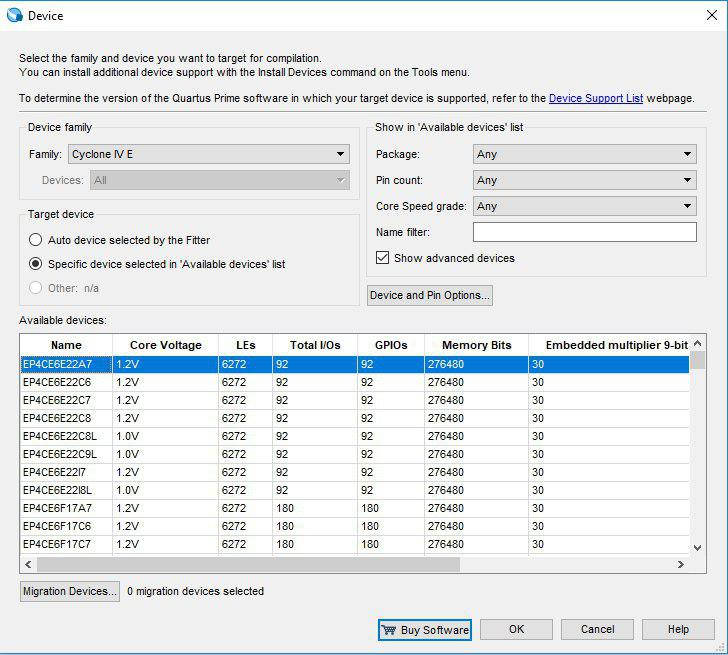
\includegraphics[width = \textwidth]{figs/synthesize/device.jpg}
\caption{انتخاب وسیله برای سنتز در محیط Quartus}
\end{figure}
\section{ایرادات سنتز و ارائهٔ راهکار}
برای شبیه‌سازی سخت‌افزاری دو ایراد وجود داشت.
\begin{itemize}
\item 
نخست این که نام ماژول و فایل یکسان نبود و ابزار 
Quartus 
در سنتز به مشکل می‌خورد.
\item 
پس از رفع ایراد پیشین ابزار هنگام سنتز اخطار زیر را می‌داد.
\begin{figure}[H]
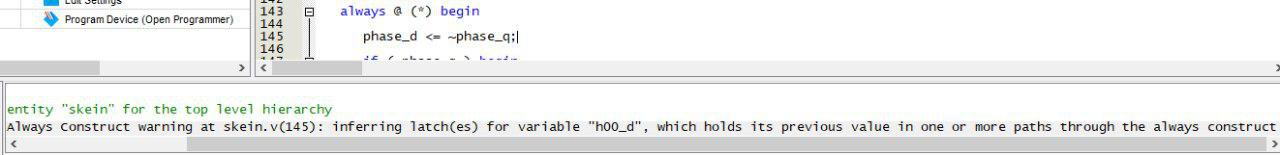
\includegraphics[width = \textwidth]{figs/synthesize/warning.jpg}
\caption{اخطار اولیه شبیه‌ساز}
\ref{warning}
\end{figure}
 برای حل این مشکل خط ۱۴۳ کد وریلاگ از 
 \begin{code}
 	always @ (*) begin
 \end{code}
 به 
 \begin{code}
 	always @ (posedge clk) begin
 \end{code}
 تغییر کرد. 
\end{itemize}

دلیل مشکل بالا این بود که یک Latch در یک بلوک ترکیبی که در آن net مقدار مشخصی نداشت تعریف شده بود و ابهام در مقدار Latch به وجود می‌آمد.


\section{گزارش پیاده‌سازی}
پس از سنتز موفق سخت‌افزاری گزارش پیاده‌سازی توسط شبیه‌ساز ارائه شد، تصاویر 
\ref{statistic_1}
و 
\ref{statistic_2}
مقادیر گزارش‌ شبیه‌ساز پس از سنتز اند.

\begin{figure}[H]
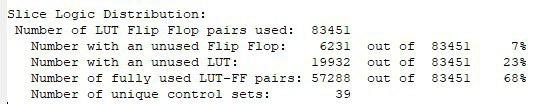
\includegraphics[scale=1]{figs/synthesize/flip_flop_pairs.jpg}
\caption{گزارش تعداد \lr{flip flop} ها و \lr{LUT} ها}
\label{statistic_1}
\end{figure}

\begin{figure}[H]
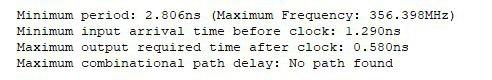
\includegraphics[scale=1]{figs/synthesize/statistics.jpg}
\caption{گزارش فرکانس و دیگر زمان‌ها در سخت‌افزار}
\label{statistic_2}
\end{figure}
